%=====================================================================
\section{Results}

\subsection{The optical reference}

\paragraph{The guide applied as is to Sentinel-2.} In the G23 forest, the guide thresholds are $m=-0.040$ and
$\sigma=0.058$ ($\Delta$NDVI). The method yields 3,349 objects of 1~ha or more (13,600~ha), i.e.
\textbf{8.7~\% of the forest in two and a half months}, while the clear-cut rate is about 1~\% per year. The
detections are mostly broadleaves, which turn yellow from September (\cref{fig-s2-overview}). The $m-k\sigma$
thresholds assume a forest that is stable between the two dates; this only holds for two summer images one
year apart, not for intra-season monitoring.

\begin{figure}[H]
\centering
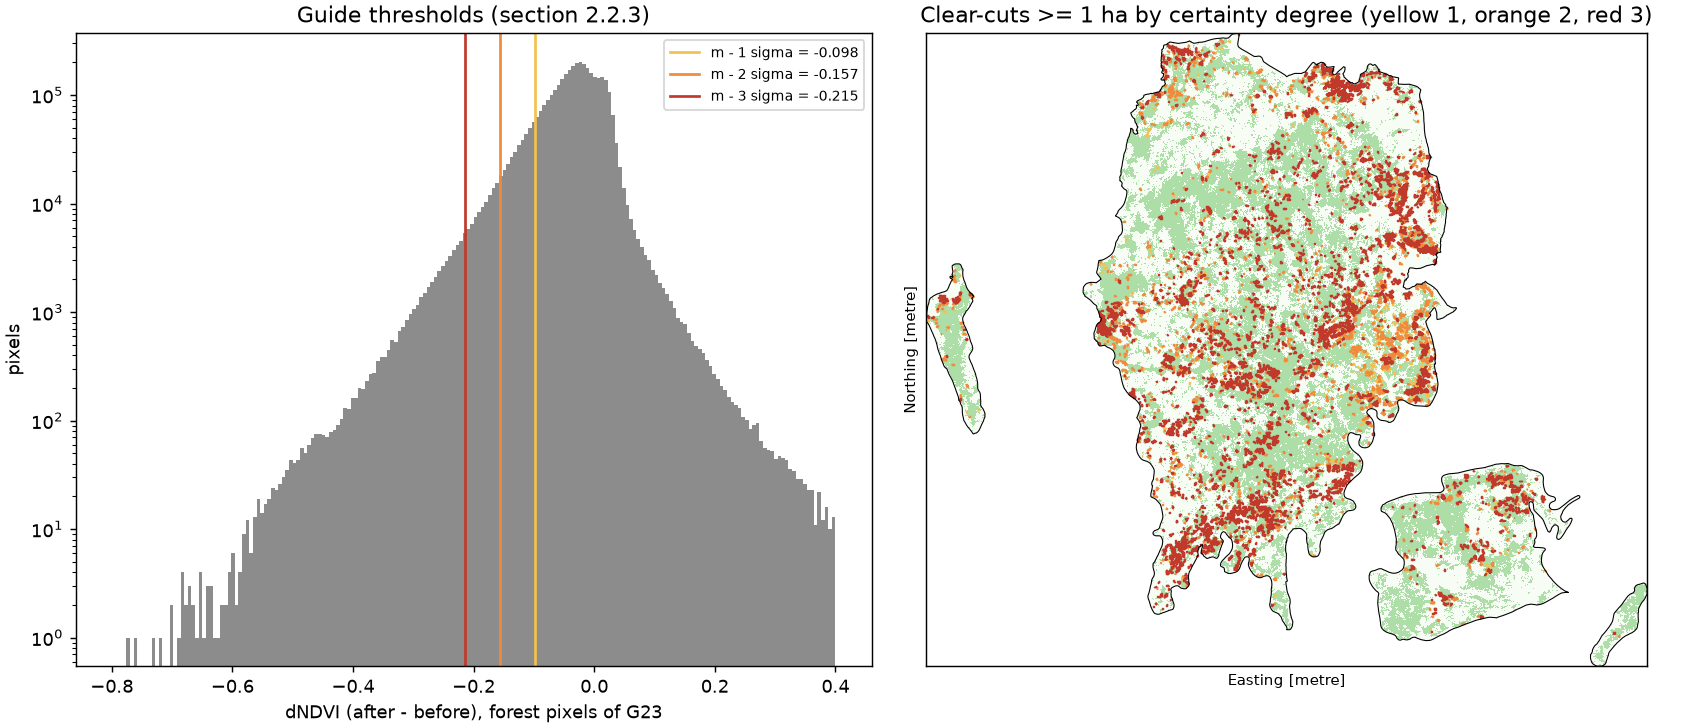
\includegraphics[width=0.9\linewidth]{s2_guide_overview.png}
\caption{The guide's method on Sentinel-2 over the whole of G23 (certainty degrees, July $\to$ September 2026).}
\label{fig-s2-overview}
\end{figure}

\paragraph{Qualified reference and photo-interpretation.} Keeping only the change from wooded to bare soil
(degree 3, NDVI before $\geq 0.70$, after $\leq 0.65$, 1~ha sieve) gives 281 cuts (613~ha). Photo-interpretation
of a sample of 30 cuts gives a precision of 59~\% (certain cuts) to 86~\% (with probable ones), on 22
interpretable objects; all errors are broadleaves. In the radar window (\cref{fig-window}), all 60 qualified cuts
were examined: only \textbf{10 show certain bare soil} (1 broadleaf, 6 conifer, 3 mixed), 9 are probable and 41
show no bare soil (senescence, shadow, thinning). The \enquote{forest before} test (July SWIR) removes three cuts
that were already open in July. The main reference therefore has \textbf{7 closed-stand cuts (15.4~ha)}.

\begin{figure}[H]
\centering
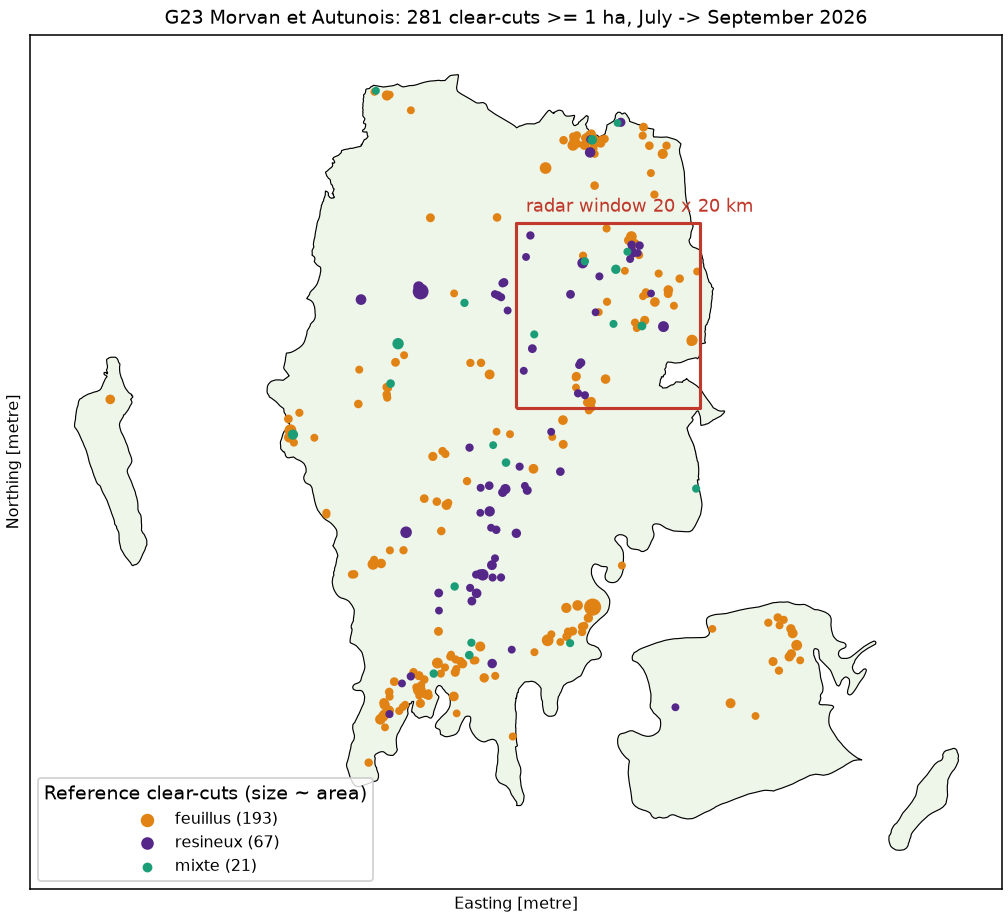
\includegraphics[width=0.8\linewidth]{s2_reference_window.png}
\caption{The $20\times20$~km radar window and the Sentinel-2 reference cuts.}
\label{fig-window}
\end{figure}

\subsection{Cut / forest separability at equal geometry}

\Cref{tab-core} and \cref{fig-summary} compare the two bands at equal geometry.

\begin{table}[H]
\centering\small
\caption{Cut / intact forest AUC [95~\% CI, cluster bootstrap], 7 closed-stand cuts.}
\label{tab-core}
\resizebox{\linewidth}{!}{\begin{tabular}{lcccc}
\toprule
Indicator & L A173 & C A59 & L D66 & C D37 \\
\midrule
$\Delta\gamma^0$ cross-pol & 0.80 {\scriptsize [0.61--0.93]} & 0.73 {\scriptsize [0.65--0.86]} & 0.83 {\scriptsize [0.66--0.93]} & 0.83 {\scriptsize [0.78--0.91]} \\
$\Delta\gamma^0$ co-pol & 0.70 {\scriptsize [0.60--0.86]} & 0.63 {\scriptsize [0.53--0.77]} & 0.71 {\scriptsize [0.60--0.82]} & 0.74 {\scriptsize [0.67--0.82]} \\
$\gamma^0$ after, cross-pol & 0.89 {\scriptsize [0.87--0.91]} & 0.76 {\scriptsize [0.72--0.84]} & 0.85 {\scriptsize [0.81--0.91]} & 0.82 {\scriptsize [0.75--0.89]} \\
minimum coherence (co-pol) & 0.60 {\scriptsize [0.53--0.66]} & 0.51 {\scriptsize [0.50--0.55]} & 0.81 {\scriptsize [0.75--0.86]} & 0.52 {\scriptsize [0.50--0.55]} \\
coherence after (co-pol) & 0.66 {\scriptsize [0.51--0.76]} & 0.68 {\scriptsize [0.61--0.79]} & 0.54 {\scriptsize [0.50--0.78]} & 0.74 {\scriptsize [0.66--0.83]} \\
\bottomrule
\end{tabular}
}
\end{table}

\begin{figure}[H]
\centering
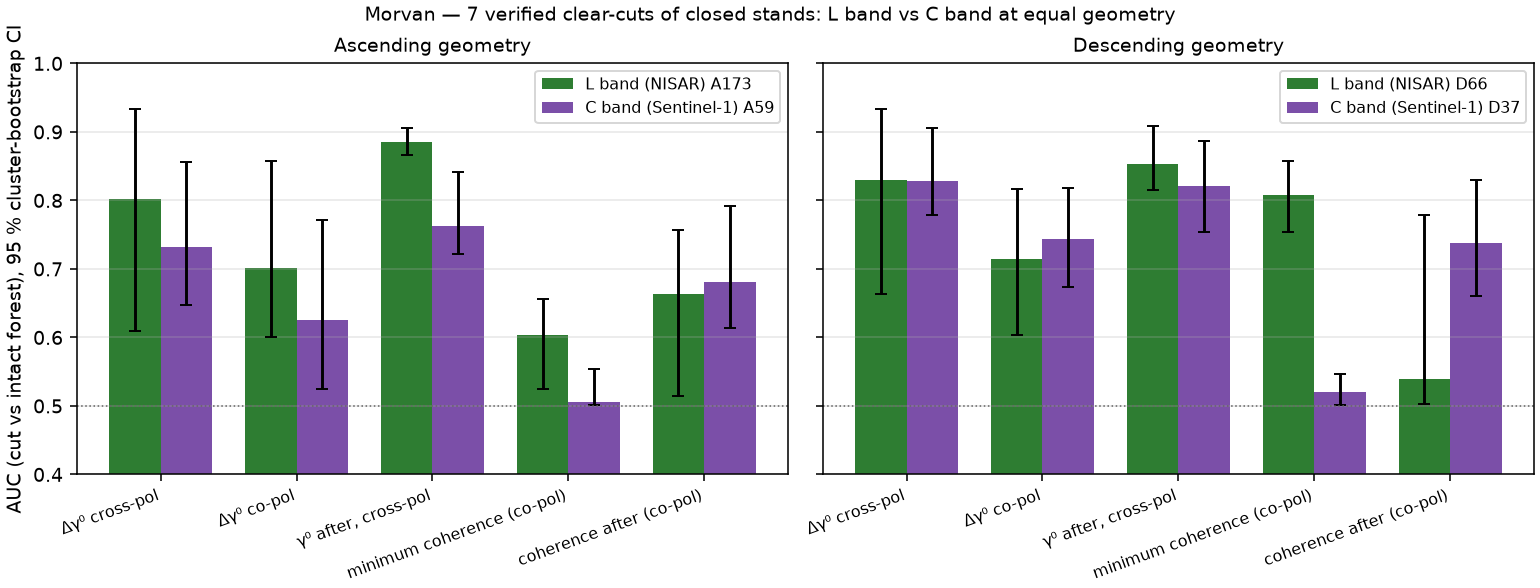
\includegraphics[width=\linewidth]{m8_summary_L_vs_C.png}
\caption{AUC of the five key indicators, L band (green) vs C band (purple), ascending and descending.}
\label{fig-summary}
\end{figure}

\begin{table}[H]
\centering\small
\caption{Cut / intact forest means.}
\label{tab-means}
\begin{tabular}{lcccc}
\toprule
Cut / intact forest & L A173 & C A59 & L D66 & C D37 \\
\midrule
cross-pol $\Delta\gamma^0$ (dB) & -2.49 / -0.23 & -1.76 / -0.44 & -2.66 / -0.33 & -2.59 / -0.60 \\
min. coherence & 0.28 / 0.32 & 0.20 / 0.21 & 0.34 / 0.48 & 0.16 / 0.16 \\
\bottomrule
\end{tabular}

\end{table}

\begin{itemize}
\item \textbf{Cross-pol backscatter.} The drop is larger in L band ($-2.5$ and $-2.7$~dB against $-1.8$ and
  $-2.6$~dB in C), and Cohen's d is larger (1.89 and 2.13 against 1.03 and 1.63). The AUC is better in L in
  ascending (0.80 vs 0.73) and equal in descending (0.83). With 7 cuts the CIs overlap: no backscatter AUC
  difference is significant.
\item \textbf{Polarisation.} Cross-pol separates better than co-pol in all four geometries (H4).
\item \textbf{Pre-cut check.} Change variables stay close to chance (AUC 0.50 to 0.57). Pre-cut level variables
  reach 0.54 to 0.64 (0.70 to 0.75 with the \enquote{verified} reference): the cut plots are special stands,
  mostly mature conifers. The post-cut $\gamma^0$ (AUC 0.85 to 0.89) is therefore partly inflated by stand
  type; the main indicator remains the change $\Delta\gamma^0$.
\item \textbf{Edge pixels.} With objects eroded by 20~m, every AUC rises by 0.03 to 0.07, without changing the
  L / C order.
\end{itemize}

\subsection{Interferometric coherence}

\begin{table}[H]
\centering\small
\caption{Median co-pol coherence of intact forest and of the cuts after the cut, over all 12-day pairs (24 days
for one NISAR pair per geometry).}
\label{tab-coh}
\begin{tabular}{lcc}
\toprule
Geometry & Intact forest & Cuts, after the cut \\
\midrule
L A173 & 0.35 -- 0.70 & 0.41 -- 0.74 \\
L D66 & 0.48 -- 0.71 & 0.59 -- 0.71 \\
C A59 & 0.30 -- 0.36 & 0.34 -- 0.53 \\
C D37 & 0.25 -- 0.27 & 0.27 -- 0.38 \\
\bottomrule
\end{tabular}
\end{table}

In C band the forest stays at the estimator floor (0.25 to 0.36 for a $10\times3$ window): it is fully
decorrelated after 12 days, as in the Vosges. In L band it keeps 0.5 to 0.7 (\cref{tab-coh}, H1). A cut
therefore becomes an event: in D66 the minimum coherence of the cuts drops to 0.34 against 0.48 for the forest
(AUC 0.81 against 0.52 in C D37). The 29/08 $\to$ 10/09 pair, which brackets three cuts, gives 0.45 on the cuts
and 0.63 in the forest.

In ascending (A173) the advantage is small (AUC 0.60): two pairs of the cut window (13/08 $\to$ 25/08 and
25/08 $\to$ 06/09) decorrelate the whole forest (0.35), probably because of a rain or wind episode, which we did
not check. Finally, in C band the cut only shows \emph{afterwards}: bare soil becomes slightly coherent in
October--November (up to 0.53) while the forest stays at the floor. Hence a higher post-cut coherence AUC in C
(0.68--0.74) than in L (0.54--0.66), but 4 to 8 weeks after the cut.

\subsection{The guide's method transposed to radar}

\begin{table}[H]
\centering\small
\caption{The guide's method on cross-pol $\Delta\gamma^0$ (best degree per geometry): area confusion matrix, share
of cuts found (at least 25~\% of their pixels) and false alarms as a share of the forest.}
\label{tab-guide}
\resizebox{\linewidth}{!}{\begin{tabular}{lllrrrcr}
\toprule
Geometry & Variable & Degree & Omission (\%) & Commission (\%) & Kappa & Objects found & False alarms (\% forest) \\
\midrule
L A173 & d\_g0\_HV & $\geq$2 & 55 & 62 & 0.41 & 5/7 & 0.09 \\
C A59 & d\_g0\_VH & $\geq$2 & 83 & 94 & 0.08 & 3/7 & 0.32 \\
L D66 & d\_g0\_HV & $\geq$2 & 51 & 64 & 0.41 & 5/7 & 0.10 \\
C D37 & d\_g0\_VH & $\geq$3 & 84 & 83 & 0.16 & 2/7 & 0.10 \\
\bottomrule
\end{tabular}
}
\end{table}

\begin{figure}[H]
\centering
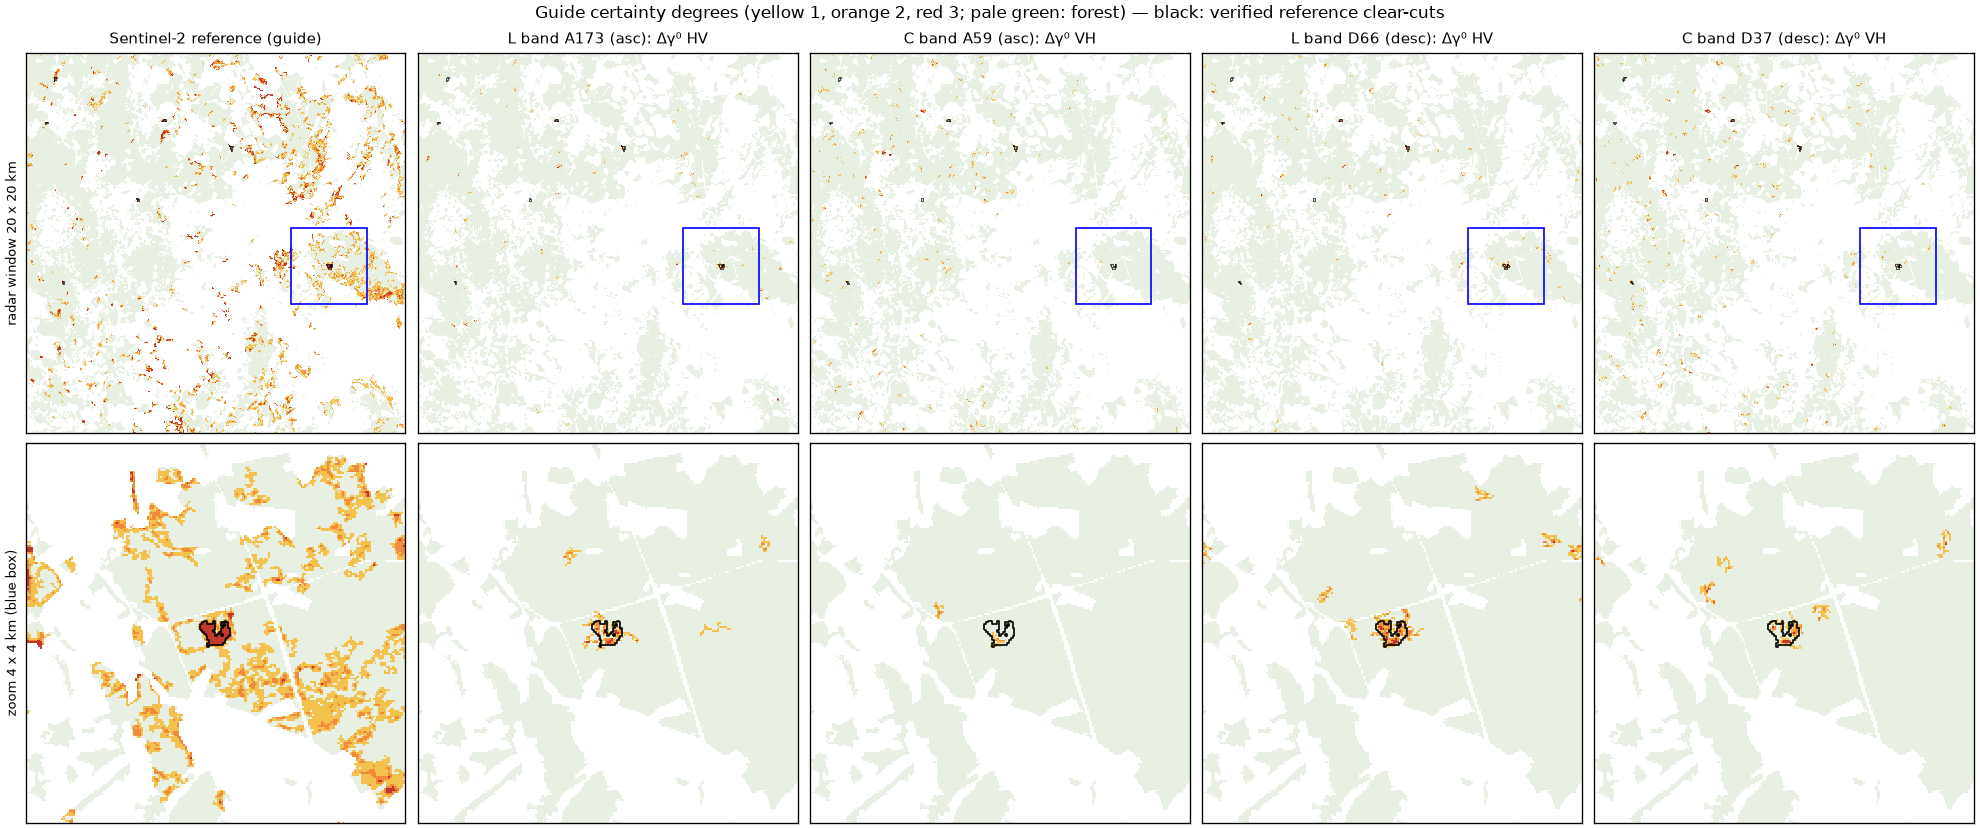
\includegraphics[width=\linewidth]{m6_guide_maps.png}
\caption{The guide's certainty degrees (yellow 1, orange 2, red 3): Sentinel-2 reference, then L band and C band
in each direction. Top: the whole window; bottom: a $4\times4$~km zoom (blue box). Black outline: verified
reference cuts.}
\label{fig-guide-maps}
\end{figure}

L band transposes the guide's method much better: kappa 0.41 and 5 of 7 cuts found in both directions, against a
kappa of 0.08 to 0.16 and 2 to 3 cuts in C band (\cref{tab-guide}, \cref{fig-guide-maps}). At the same degree
($\geq 2$), L band produces 11 to 13~ha of false alarms over 12,800~ha evaluated (0.1~\% of the forest), C band 41
to 52~ha. This holds for all four references (\cref{tab-refs-guide}). We remain, however, far from the guide's
target (10~\% omission and commission): 51 to 55~\% omission and 62 to 64~\% commission in L.

\begin{table}[H]
\centering\small
\caption{Kappa of the guide's method (best combination) by reference.}
\label{tab-refs-guide}
\begin{tabular}{lcccc}
\toprule
Reference (objects) & L A173 & C A59 & L D66 & C D37 \\
\midrule
automatic (60) & 0.13 & 0.04 & 0.13 & 0.09 \\
verified + probable (19) & 0.27 & 0.07 & 0.27 & 0.15 \\
verified (10) & 0.34 & 0.08 & 0.34 & 0.19 \\
closed stands (7) & 0.41 & 0.08 & 0.41 & 0.16 \\
\bottomrule
\end{tabular}
\end{table}

\paragraph{False alarm audit.} The 15 largest objects detected by NISAR D66 outside any known cut were
photo-interpreted (\cref{fig-audit}). Two are probable late cuts (F01, 2.5~ha; F04, 1.6~ha), cut after the
Sentinel-2 \enquote{after} window; the other 13 are senescence, edges, larch yellowing or hedgerows. The same
audit on Sentinel-1 D37 (\cref{fig-audit-s1}; VH $\Delta\gamma^0$, degree 3) finds \textbf{no late cut}: 8 of 15
objects (22 of 36~ha) are plots already open in June (old cuts, heathland, meadows still mapped as closed forest
by BD Forêt), where the low vegetation changes (senescence, soil work); the other 7 are intact forest, edges or
senescence. C band reacts to low vegetation, as on cuts R019, R139 and R225, which were open before July; L band
does not.

\begin{figure}[H]
\centering
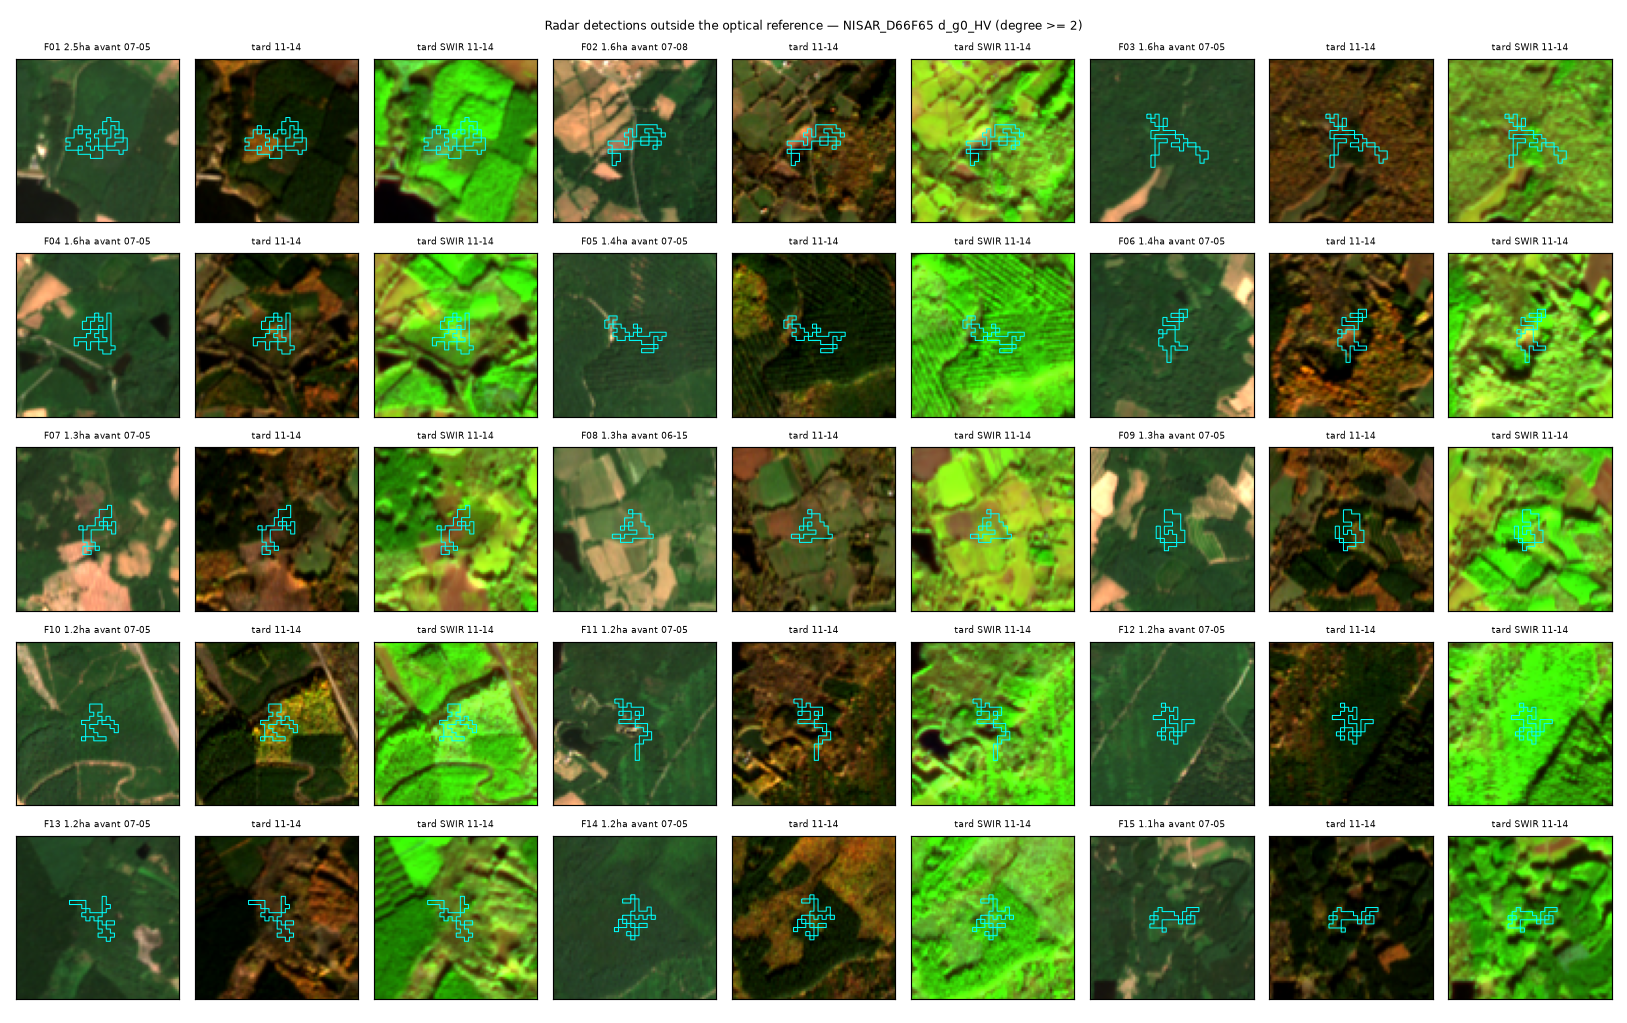
\includegraphics[width=\linewidth]{m6b_commission_NISAR_D66F65_d_g0_HV.png}
\caption{Audit of the 15 largest NISAR D66 false alarms: Sentinel-2 in July, in November (true colour) and in
November (SWIR / NIR / red).}
\label{fig-audit}
\end{figure}

\begin{figure}[H]
\centering
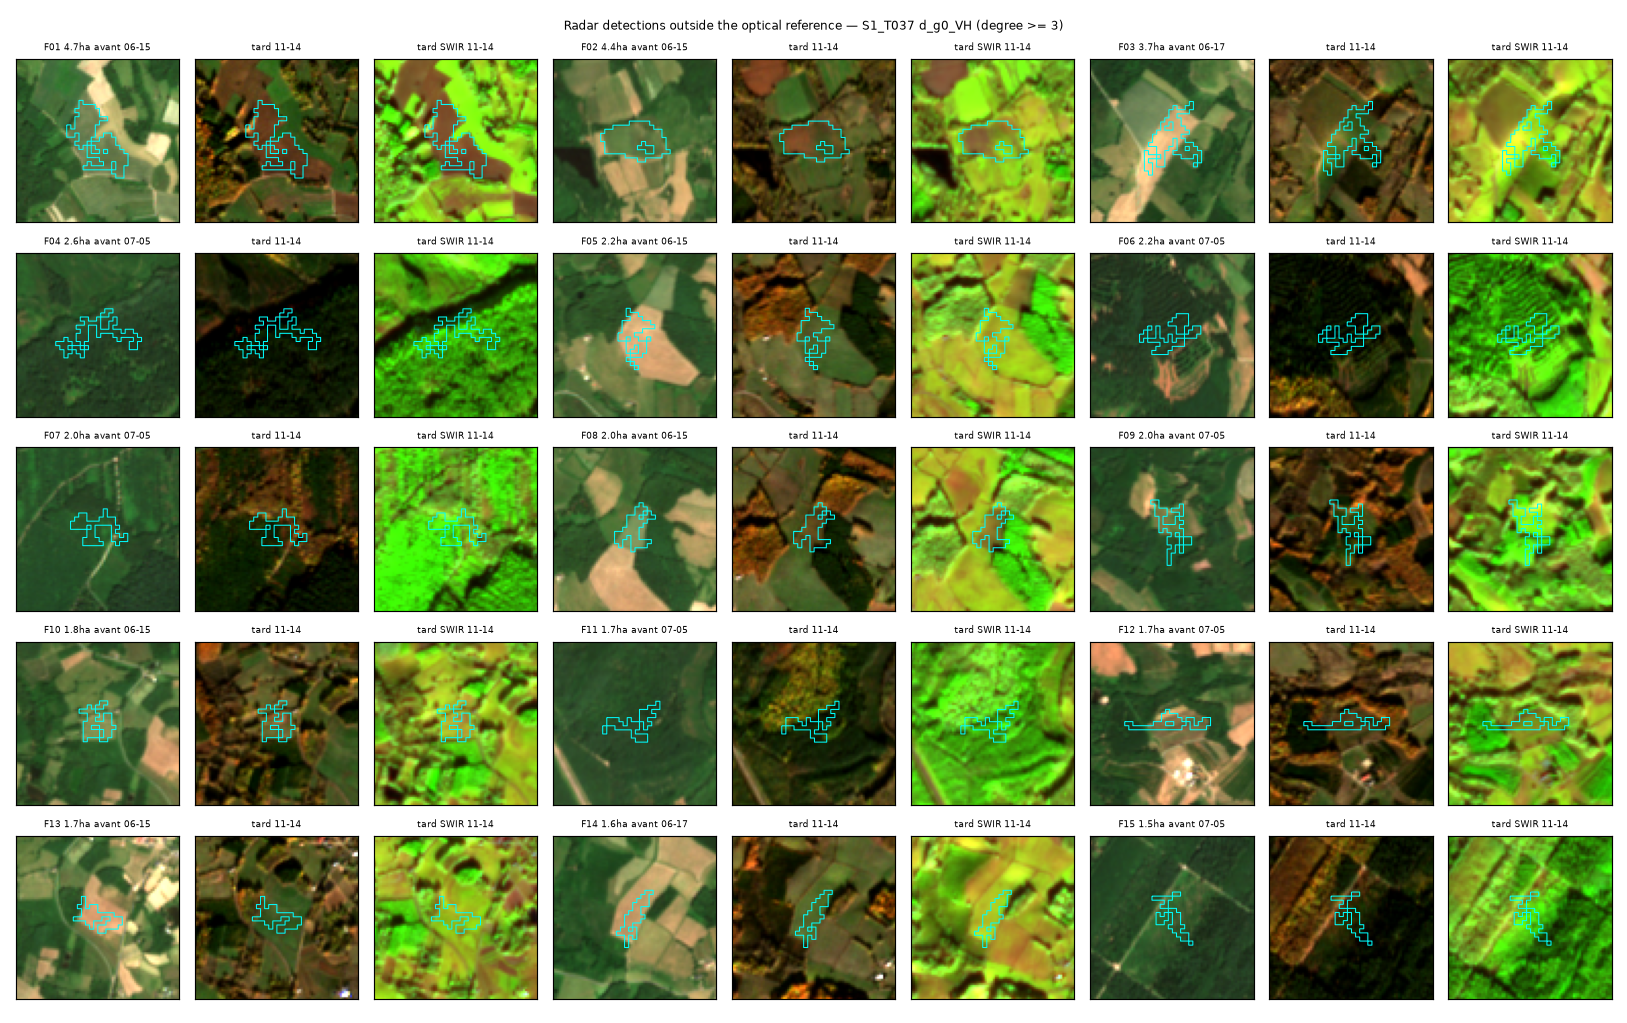
\includegraphics[width=\linewidth]{m6b_commission_S1_T037_d_g0_VH.png}
\caption{Audit of the 15 largest Sentinel-1 D37 false alarms (same chips).}
\label{fig-audit-s1}
\end{figure}

\subsection{Sensitivity to the reference}

\begin{table}[H]
\centering\small
\caption{AUC of cross-pol $\Delta\gamma^0$ by reference.}
\label{tab-refs}
\begin{tabular}{lcccc}
\toprule
Reference (objects) & L A173 & C A59 & L D66 & C D37 \\
\midrule
automatic (60) & 0.56 & 0.51 & 0.56 & 0.53 \\
verified + probable (19) & 0.63 & 0.61 & 0.63 & 0.67 \\
verified (10) & 0.68 & 0.70 & 0.71 & 0.78 \\
stand (7) & 0.80 & 0.73 & 0.83 & 0.83 \\
\bottomrule
\end{tabular}

\end{table}

Reference quality dominates everything else (\cref{tab-refs}): the AUC rises from 0.51--0.56 with the automatic
reference to 0.73--0.83 with the 7 closed-stand cuts. Without photo-interpretation, we would have wrongly
concluded that neither L nor C band sees the cuts. The L / C order, however, depends on the reference: with the
\enquote{verified} references, C band equals or exceeds L band (0.78 vs 0.71 in descending). These references
include three plots already open in July (R019, R139, R225): their L-band HV was already low and drops little
(less than 1.3~dB), whereas C band, sensitive to low vegetation and slash, drops by 1.7 to 3.9~dB. L band
responds to the loss of trunks, C band to any change of the low layer. This is why the main reference is
restricted to closed stands.

\subsection{Radar dating of the cuts}

\begin{table}[H]
\centering\small
\caption{Cut interval (first lasting cross-pol drop of more than 2~dB), closed-stand cuts; R: conifer, M: mixed,
F: broadleaf.}
\label{tab-dating}
\begin{tabular}{lcccc}
\toprule
Cut & L A173 & C A59 & L D66 & C D37 \\
\midrule
R013 (R, 5.1 ha) & 25/08--06/09 & -- & 29/08--10/09 & 25/08--06/09 \\
R060 (M, 2.9 ha) & 25/08--06/09 & 09/07--21/07 & 29/08--10/09 & 25/08--06/09 \\
R100 (R, 2.1 ha) & -- & 07/09--19/09 & -- & 06/09--18/09 \\
R144 (R, 1.6 ha) & -- & -- & -- & 25/08--06/09 \\
R161 (F, 1.4 ha) & 06/09--18/09 & 07/09--19/09 & 29/08--10/09 & 06/09--18/09 \\
R198 (M, 1.3 ha) & 20/07--13/08 & 21/07--02/08 & 24/07--17/08 & 25/08--06/09 \\
R246 (R, 1.1 ha) & 20/07--13/08 & 14/08--26/08 & 12/07--24/07 & 25/08--06/09 \\
\bottomrule
\end{tabular}

\end{table}

\begin{figure}[H]
\centering
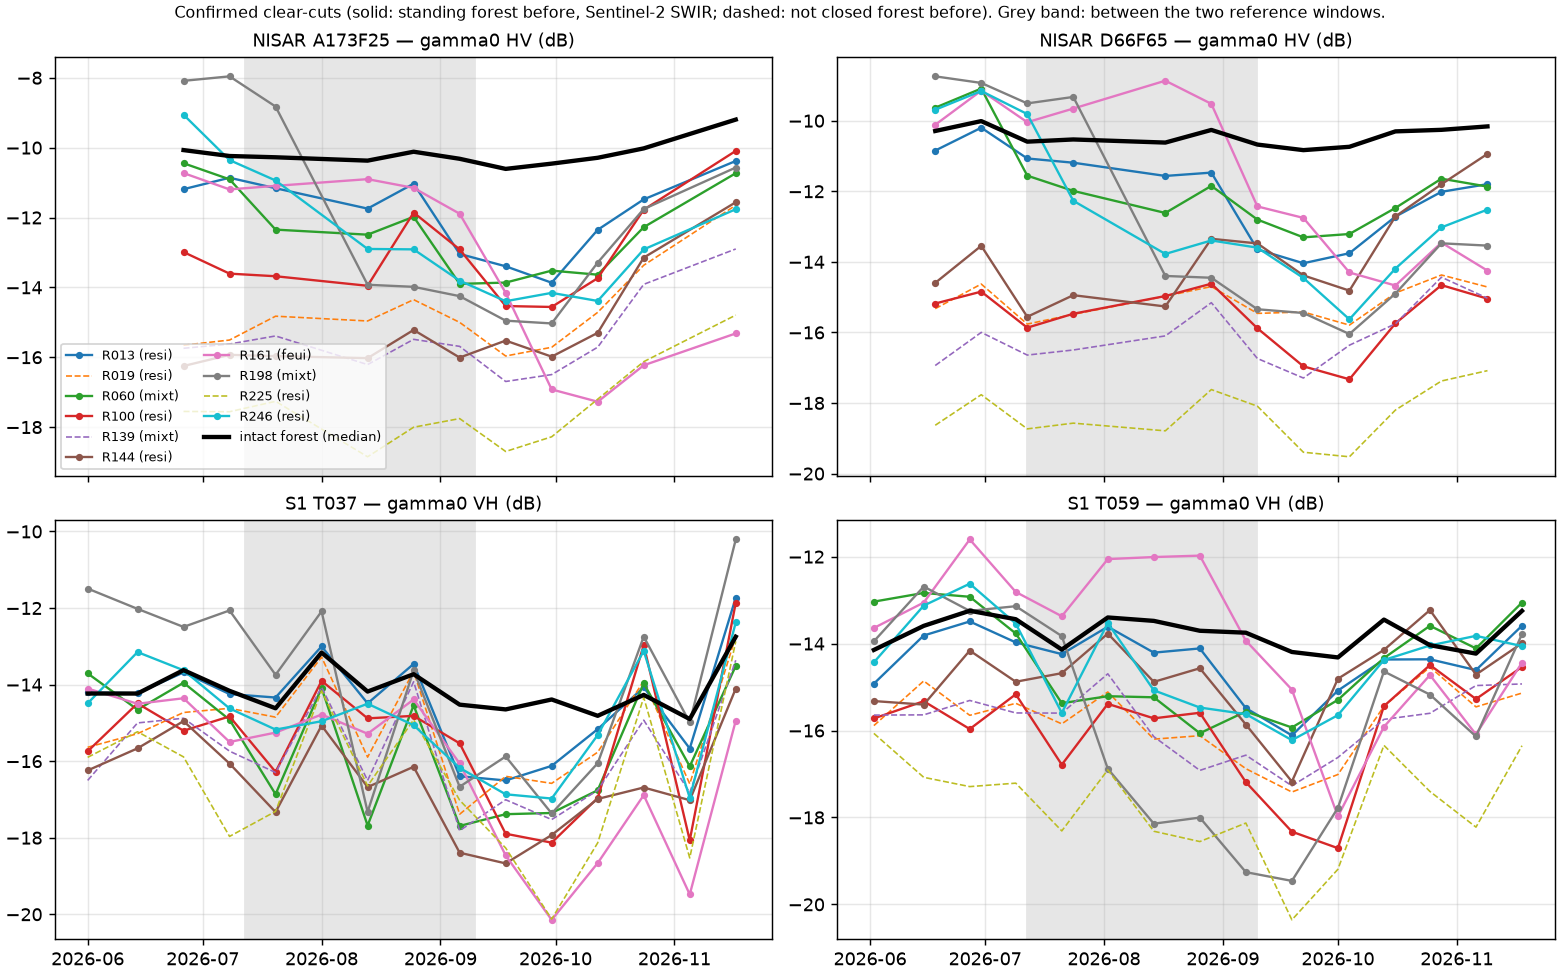
\includegraphics[width=\linewidth]{m7_cut_timeseries.png}
\caption{Cross-pol $\gamma^0$ series of the confirmed cuts and median of intact forest.}
\label{fig-ts}
\end{figure}

In L band the series are smooth and both geometries agree (\cref{tab-dating}, \cref{fig-ts}): R013 and R060 late
August -- early September, R161 early September, R198 and R246 late July -- mid-August. In C band, orbit D37 shows
synchronous $\pm3$~dB jumps over the whole forest, probably linked to moisture; it puts 5 of the 7 cuts in the
same pair, which is not credible. The more stable orbit A59 narrows the date of R198 (21/07 -- 02/08). R100 is
only detected in C band (September, in both orbits); in L band the drop stays below 2~dB. Thinning or late
skidding, to which C band reacts more, is the simplest hypothesis.

\subsection{Hypotheses}

\begin{table}[H]
\centering\small
\caption{Hypotheses on the Morvan.}
\label{tab-hyp}
\begin{tabular}{lp{10.5cm}l}
\toprule
H & Finding & Verdict \\
\midrule
H1 & Intact forest: coherence 0.5--0.7 in L against 0.25--0.36 in C (floor). & confirmed \\
H2 & D66: AUC 0.81 against 0.52 in C; A173: 0.60 (forest-wide decorrelation in late August). & partial \\
H3 & Larger drop in L (Cohen's d 1.9--2.1 against 1.0--1.6); AUC L $\geq$ C, not significant. & partial \\
H4 & Cross-pol $>$ co-pol in both bands and all four geometries. & confirmed \\
\bottomrule
\end{tabular}
\end{table}

%=====================================================================
\section{Discussion}

\paragraph{Comparison with the Vosges.} Both sites give the same message. The forest stays coherent in L band
(0.64--0.70 in the Vosges, 0.5--0.7 here) and not in C band (0.28 and 0.25--0.36). The L-band backscatter
advantage depends on geometry: in the Vosges it only existed in ascending; here the AUC is better in ascending
and equal in descending. The replication removes the two limits of the first test (a single cut, a single
Sentinel-1 orbit) and indicates that the Vosges result was not an isolated case. On the other hand, the almost perfect coherence AUC of
the Vosges (0.995) is not found again: over 7 cuts at different dates, summer pairs are sometimes decorrelated
over the whole forest.

\paragraph{Why the guide's method favours L band.} At equal AUC (0.83 in descending), L band gives a kappa of
0.41 and C band 0.16. The AUC measures the average ranking of pixels; an $m-k\sigma$ threshold method only keeps
the tail of the distribution, where the gap in standard-deviation units matters (Cohen's d 2.13 against 1.63).
L band is also more stable from one date to the next, which narrows the forest distribution and reduces false
alarms. For an operational service based on thresholds, this is the criterion that counts.

\paragraph{The reference, the limiting factor.} The guide recommends a photo-interpretation check; this work shows
it is essential. Within a season, broadleaf senescence causes most NDVI drops: only 10 of the 60 qualified cuts of
the window are certain cuts. Radar scores measured against an automatic reference are very pessimistic lower
bounds.

\paragraph{Complementarity of the two bands.} C band reacts to events that L band barely sees (R100, probably
thinning or skidding) and its revisit sometimes narrows a date (R198). L band gives more stable series, dates that
agree between geometries and fewer false alarms. An operational detector would gain from combining both, with
temporal confirmation.

\paragraph{Limits.} Only seven cuts and 15~ha: the CIs are wide and backscatter AUC differences are not
significant. A single season, a single landscape dominated by conifer cuts. The optical reference misses late
cuts (two of them appear as radar false alarms) and cuts without bare soil. The coherence estimators differ
(NISAR GUNW vs SNAP $10\times3$), NISAR products are provisional, and the weather was not checked.

%=====================================================================
\section{Conclusion}

On seven verified clear-cuts in the Morvan and at equal geometry in both look directions:
\begin{enumerate}
\item L band keeps the forest coherent (0.5--0.7) and C band does not (floor at 0.25--0.36): H1 is confirmed on
  a second site;
\item L-band coherence separates the cuts in descending (AUC 0.81 vs 0.52), less in ascending, where a
  forest-wide decorrelation episode masks the signal;
\item in backscatter the AUCs are close (L $\geq$ C), but the contrast is stronger in L, and the guide's method
  transposed to radar works much better in L band (kappa 0.41, 5 of 7 cuts) than in C band (0.08--0.16, 2 to 3
  cuts), without reaching the 10~\% error target;
\item the quality of the optical reference dominates the results: photo-interpretation is essential.
\end{enumerate}
The chain (\texttt{nisar\_s1} package, per-site configuration) transfers directly to ROSE-L~\cite{esa2020rosel}
and to ISCE3 products~\cite{isce3}. The next step is a detector combining L coherence, L backscatter and C
revisit, evaluated over several seasons and regions.
